%FOR PDFLATEX USE ONLY
\documentclass[a4paper,12pt]{article}

\usepackage{amssymb,amsmath} %math symbols

\usepackage[margin=2cm]{geometry} %paper geometry

\usepackage[utf8]{inputenc} %allows unicode (including russian) source file
\usepackage[russian]{babel} %docment in russian-style
\usepackage[utf8]{inputenc}
%\usepackage[unicode]{hyperref} %links inside of the text
\usepackage[pdftex]{graphicx} %includegraphics pictures
\usepackage{cmlgc} %bold text

\usepackage{array} %arrays

%\usepackage{wrapfig}
%\usepackage{array}
%\usepackage{lipsum}
%\usepackage{esvect}
%\usepackage{hyperref}

\usepackage{subfig}
%\usepackage{calc}
%\usepackage{pgfplots,tikz,circuitikz}
%\usepackage{tkz-euclide}

\begin{document}

\begin{center}
  \LARGE{Работа 4.3.3}\\[0.2cm]
  \LARGE{Исследование разрешающей способности микроскопа методом Аббе}\\[0.2cm]
  \large{Стрижак Даниил}\\[0.2cm]
\end{center}  
  

\section{Аннотация}
В работе предлагается определить периоды сеток сначала по их спектру на удалённом экране, затем по увеличенному с помощью модели микроскопа изображению сеток на экране и, наконец, по результатам измерения разрешающей способности микроскопа, наблюдать явления саморепродукции, пространственной фильтрации и мультиплицирования.

\section{Теоретические сведения}

 Для иммерсионного микроскопа разрешающая способность объектива при некогерентном
освещении
$$
\ell_{\min } \approx \frac{0.61 \lambda}{n \sin u}
$$
где $u-$ апертурный угол объектива микроскопа (угол между оптической осью и лучом, направленным из центра объекта в край линзы).

Метод Аббе для оценки разрешающей способности состоит в разделении хода лучей на две части: сначала рассматривается картина в задней фокальной плоскости $F$ объектива она называется первичным изображением или фурье-образом. Это первичное изображение рассматривается как источник волн (принцип Гюйгенса-Френеля), создающий изображение в плоскости $P_{2}$, сопряжённой плоскости предмета - вторичное изображение. Первичное изображение есть картина дифракции Фраунгофера (на дифракционной решётке $),$ если её период $d$, то для направления максимальной интенсивности $\varphi_{m}$
$$
d \sin \varphi_{m}=m \lambda
$$
При этом проходят пучки только с $\varphi_{m}<u .$ Можно условием разрешения считать, что $u>\varphi_{1}$, иначе говоря
$$
\sin u \geq \lambda / d
$$
Или
$$
d \geq \frac{\lambda}{\sin u} \approx \frac{\lambda}{D / 2 f}
$$
где $D-$ диаметр линЗы, $f-$ фокусное расстояние. Двумерную решётку можно рассматривать как две перпендикулярные друг другу, для максимумов которых выполняется соотношение
$$
d \sin \varphi_{x}=m_{x} \lambda, \quad d \sin \varphi_{y}=m_{y} \lambda
$$


\newpage
\subsection*{Установка}

\begin{center}
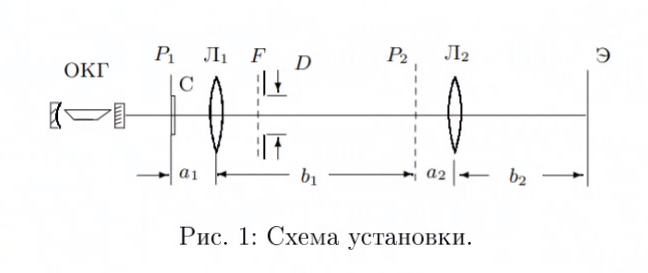
\includegraphics[width = 0.7\textwidth]{1.jpeg}
\end{center}

Схема установки приведена на Рис. 1. Предметом $P_{1}$ служат сетки в кассете $C .$ \\Линза Л1 -- длиннофокусная, а Л2 -- короткофокусная. В F Устанавливаются диафрагмы D, с помощью сеток с разными $d$ и щелевой диафрагмы можно проверить третье соотношение. Период сеток может быть измерен либо по расстоянию между дифракционными максимумами на экране, либо по увеличенному с помощью микроскопа изображению сетки на экране. Пространственную фильтрацию (получение наклонного изображение решётки) можно получить с помощью подбора угла наклона и ширины вспомогательной щели.

\section{Результаты измерений и обработка данных}

\subsection*{I. Определение периода решёток по их пространственному спектру}

Соберём установку согласно описанию. Длина волны излучения лазера $\lambda=532 \mathrm{нм}$
Расстояние от сетки до экрана $H=100 \pm 2$ см, погрешность объясняется неопределённостью положения сетки внутри кассеты, погрешностью меток на столе, использованных при измерении, и погрешностью прямого измерения. Измерим линейкой на экране расстояние $\Delta x$ между $n+1$ максимумами и рассчитаем по второй формуле с учётом $\varphi=\frac{\Delta x}{H}$ период решетки $d = \frac{n\lambda}{\Delta x}H$. Результаты приведены в Таблице $1 .$

\begin{minipage}{0.47\textwidth}
\begin{center}
\begin{tabular}{|c|c|c|c|}
\hline
Номер &$\Delta x$, см &  n&$d$, мкм\\
решётки&		&			& \\
\hline
1 &	22.7	&6	& 		20	\\
\hline
2&	22.6	&	9	&	30		\\
\hline
3&	25.1	&20		&	60		\\
\hline
4&	22.5	&	35	&	117		\\
\hline
5&	22.7	&	48	&		159	\\
\hline
\end{tabular}
\newline
\newline
Таблица 1. 
\end{center}
\end{minipage}
\begin{minipage}{0.47\textwidth}
\begin{center}
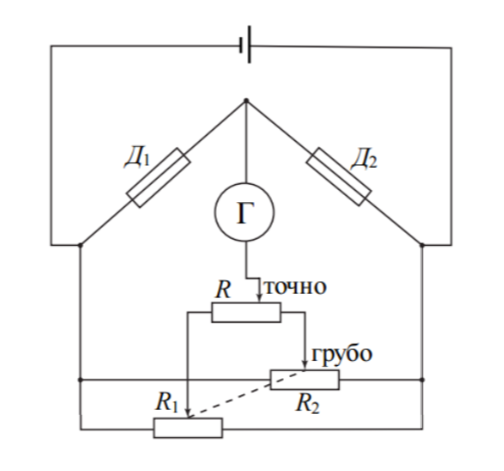
\includegraphics[width = \textwidth]{2.JPG}
\end{center}

\begin{center}
Дифракция Фраунгофера на двумерной решетке.
\end{center}
\end{minipage}



 
\subsection*{II. Определение периода решёток по изображению, увеличенному с помощью модели микроскопа}
  
Соберём модель микроскопа, добавив линзы согласно Рис. 1. Фокусные расстояния линз $F_{1}=  $ мм, $F_{2}= $ мм. Измеряем необходимые расстояния:
$$
\begin{aligned}
a_{1} &= 120  \pm 10 \mathrm{мм}, \\
a_{2}+b_{1} &= 455 \pm 10 \mathrm{см}, \\
b_{2} &= 815 \pm 10 \mathrm{см},
\end{aligned}
$$
Погрешности здесь обусловлены неточностями в положенияъ сеток и линз. Из формулы тонкой линзы \fbox{$a_{2}=\frac{b_{2} F_{2}}{b_{2}-F_{2}}=25.79$ мм}, откуда \fbox{$a_{2} \approx F_{2}$}, поэтому в дальнейшем будем использовать это значение, следовательно $b_{1}= 420\pm 10$ мм.  Увеличение микроскопа \fbox{$ \Gamma=\frac{b_{1} b_{2}}{a_{1} a_{2}}=114 \pm 10 .$}

Повторим измерения периодов изображений в новой конфигурации, погрешности считаются аналогично. Измерение представлены в Таблице $2 .$

Здесь $d$ определялось по формуле $d=\frac{\Delta x}{\Gamma n}$. Обратим внимание, что значения периодов решётки совпадают в пределах погрешности.

\begin{minipage}{0.47\textwidth}
\begin{center}
\begin{tabular}{|c|c|c|c|}
\hline
Номер &$\Delta x$, см &  n&$d$, мкм\\
решётки&		&			& \\
\hline
1 &	3.7	&	16	& 	20		\\
\hline
2&	15.7	&	49	&	28		\\
\hline
3&	25.3	&	38	&	58		\\
\hline
4&	24.1	&	18	&	117		\\
\hline
5&	23.6	&	13	&	159	 	\\
\hline
\end{tabular}
\newline
\newline
Таблица 2. 
\end{center}
\end{minipage}
\begin{minipage}{0.47\textwidth}
\begin{center}
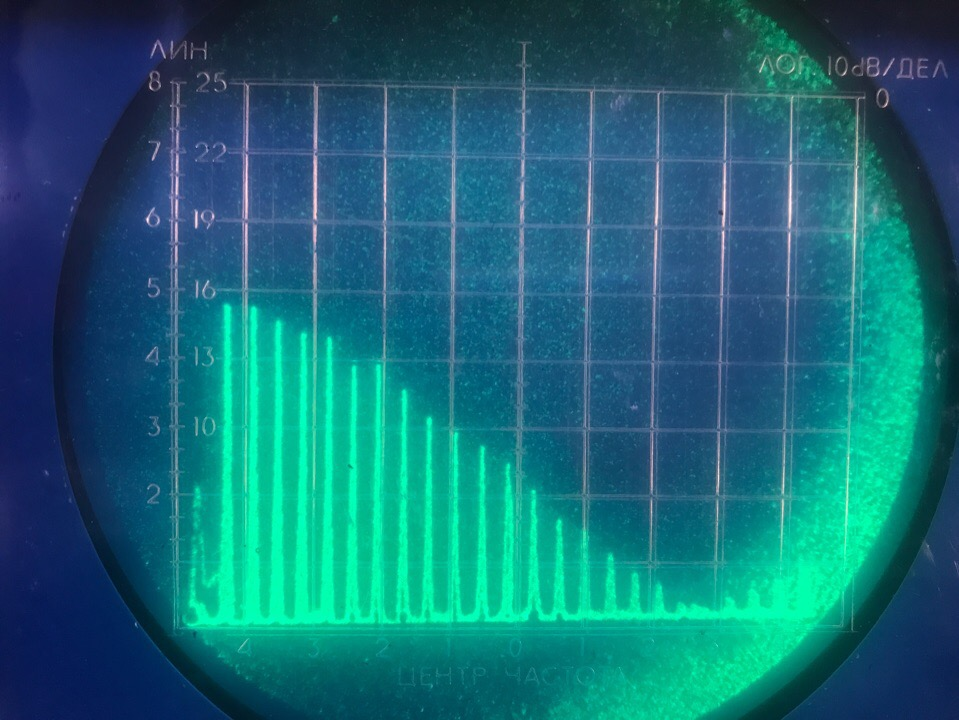
\includegraphics[width = \textwidth]{3.JPG}
\end{center}

\begin{center}
Увеличенное изображение сетки.
\end{center}
\end{minipage}

\newpage
  
\subsection*{III. Определение периода решёток по оценке разрешающей способности микроскопа}

Поместим в фокальной плоскости линзы $Л_{1}$ щелевую диафрагму с микрометрическим винтом и определим минимальную толщину $D$ при которой на экране видна двумерная решётка. В этом случае период будет вычисляться по формуле (3) в предельном случае
$$
d=\frac{2 \lambda F_{1}}{D}
$$
погрешность вычисляется по формуле
$$
\sigma_{d}=d \frac{\sigma_{D}}{D} .
$$
Результаты приведены в Таблице $3 .$



\begin{minipage}{0.47\textwidth}
\begin{center}
\begin{tabular}{|c|c|c|c|}
\hline
Номер &D , мм &  1/D, мм&$d$, мкм\\
решётки&		&			& \\
\hline
1 &--		&	--	& 		--	\\
\hline
2&	4.14	&	0.242	&	28.3		\\
\hline
3&	1.96	&	0.510	&	59.7		\\
\hline
4&	1.02	&	0.980	&	114.7		\\
\hline
5&	0.81	&	1.240	&		144.5	\\
\hline
\end{tabular}
\newline
\newline
Таблица 3. 
\end{center}
\end{minipage}
\begin{minipage}{0.47\textwidth}
\begin{center}
		\begin{tikzpicture}[scale = 1.0]
		\begin{axis}[
		axis lines = left,
		ylabel = {d, мкм},
		xlabel = {1/D, мм},
		minor grid style={black, line width=0.05pt},
		major grid style={solid,black, line width=0.3pt},
		xmin=0, xmax=1.4,
		ymin=0, ymax=160,
		ymajorgrids = true,
		xmajorgrids = true,
		yminorgrids = true,
		xminorgrids = true,
		minor tick num = 4
		]
		\addplot+[only marks ] plot[error bars/.cd, y dir=both, y explicit]
		coordinates {
			(0.242,28.3)
			(0.510,59.7)
			(0.980,114.7)
			(1.24,144.5)
		};
		
		\addplot[blue, domain=0:8]{120.43*x };
		\end{axis}

		\end{tikzpicture}

Зависимость $d=f(1 / D)$. 
		
\end{center}
\end{minipage}

\newline
\
\newline


Через щель проходили только нулевой (по центру) и два первых максимумы, за исключением второй щели, где нулевой максимум был помещён к краю щели. Для первой решётки
период таким методом измерить не получилось, так как ширины щели не хватает.

Для проверки теории Аббе построим график $d=f\left(\frac{1}{D}\right)$ со значениями $d$ из части 1, погрешность $\frac{1}{D}$ рассчитывается по формуле
$$
\sigma_{1 / D}=\frac{\sigma_{D}}{D^{2}}
$$
Угловой коэффициент прямой из $\mathrm{MHK}\ k=(124 \pm 8) \cdot 10^{-9} м^{2}$, в пределах погрешности он совпадает с теоретическим $2 \lambda F_{1}= 117\cdot 10^{-9} м^{2} .$ Таким образом, теория Аббе подтвердилась. 


\newpage
   
 \subsection*{IV. Пространственная фильтрация и мультиплицирование}
 
 Для наблюдения фильтрации на сетке 2 откроем щель так, чтобы она пропускала только максимум нулевого порядка и, поворачивая щель, наблюдаем за изменением картины. Картины представлены на рисунках ниже. \\
 
 \begin{minipage}{0.47\textwidth}
\begin{center}
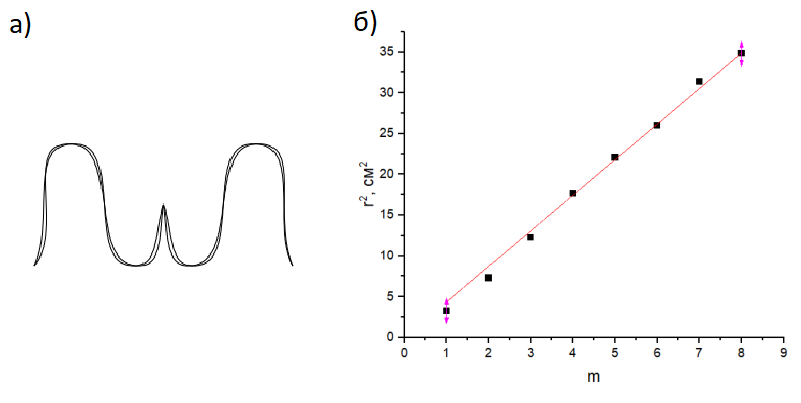
\includegraphics[width = \textwidth]{4.JPG}
\end{center}

\begin{center}
Горизонатальная щель $\left(0, m_{y}\right)$. 
\end{center}
\end{minipage}
\begin{minipage}{0.47\textwidth}
\begin{center}
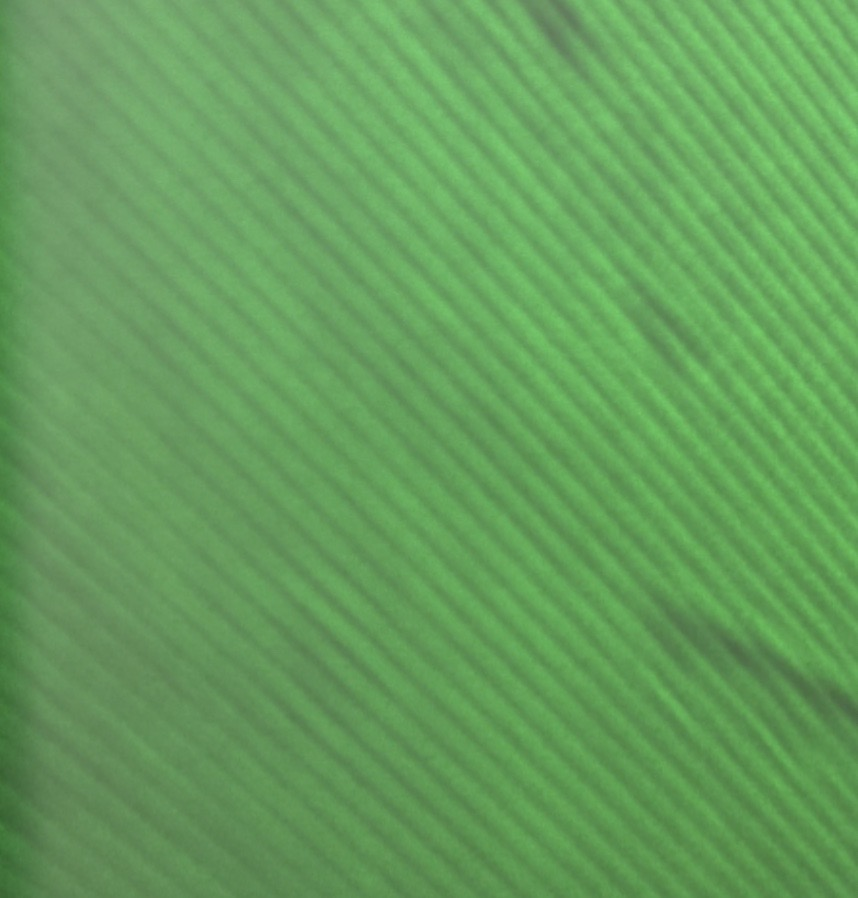
\includegraphics[width = 0.95\textwidth]{6.JPG}
\end{center}

\begin{center}
Щель, повернутая на $45^{\circ}\left(m_{x}=m_{y}\right)$. 
\end{center}
\end{minipage}
 
 
 \begin{minipage}{0.47\textwidth}
\begin{center}
 Для наблюдения мультиплицированния поменяем местами сетку и щель, пронаблюлюдаем мультипликацию, картина представлена на Рис. $4 .$

\end{center}
\end{minipage}
\begin{minipage}{0.47\textwidth}
\begin{center}

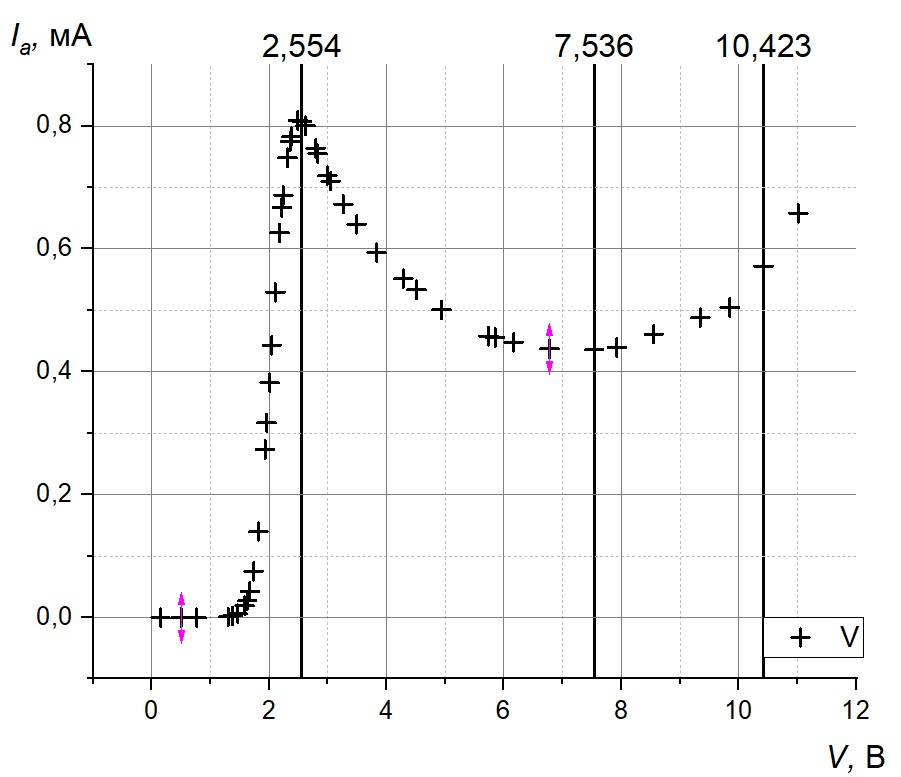
\includegraphics[width = \textwidth]{5.JPG}
\end{center}

\begin{center}
Схема для наблюдения интерфереционной картины.

\end{center}
\end{minipage}
\section{Вывод}


По измерениям спектров получилось определить дифракционные углы и по теоретическим формулам рассчитали периоды решеток. Полученные данные сошлись с результатами,  полученными по измерениям увеличенных с помощью микроскопа изображений сеток. Построив график зависимости d = f(1/D), взяв периоды сеток, определённые по спектру мы убедились в справедливости теории Аббе. 


\end{document}
